\documentclass[16pt]{beamer}
\usepackage[utf8]{inputenc}
\usepackage{media9}
\usepackage{amsmath}
\usepackage{amsfonts}
\usepackage{amssymb}
\usepackage{amsthm}
\usepackage{graphicx,epsfig}
\usepackage{xcolor}
 
\usetheme{Madrid}
\usecolortheme{beaver}

\usepackage{anyfontsize}
 
%Information to be included in the title page:
\title[Stability of Multi-Pulses]{Stability of Multi-Pulse Solutions to the 5th order Korteweg–de Vries (KdV) Equation}
\author[R. Parker]{Ross Parker, Bj\"{o}rn Sandstede}
\institute{Brown University}
\date{Sometime in May}

\AtBeginSection[]
{
  \begin{frame}
    \frametitle{Outline}
    \tableofcontents[currentsection]
  \end{frame}
}
 
\begin{document}
 
\frame{\titlepage}
 
\begin{frame}
\frametitle{Outline}
\tableofcontents
\end{frame}

\section{Background}

\begin{frame}
	\frametitle{Fifth-order KdV Equation }   
	\fontsize{16}{7.2}\selectfont
	\begin{center}
		\[ u_t = u_{xxxxx} - u_{xxx} - 2 u u_x \]
	\end{center}
	\vspace{0.5cm}
	Weakly nonlinear long wave approximation to capillary-gravity wave problem
	\vspace{0.5cm}
	\begin{itemize}
		\item Long wave (Boussinesq) approximation
		\begin{itemize} 
			\item Wavelength long compared to wave depth
		\end{itemize}
		\item Capillary-gravity waves
		\begin{itemize}
		    \item Influenced by surface tension and gravity
		    \item Longer wavelength than ripples
		    \item Shorter wavelength than ordinary water waves 
		\end{itemize}
	\end{itemize}
\end{frame}

\begin{frame}
	\frametitle{Fifth-order KdV Equation}
	\fontsize{16}{7.2}\selectfont
	\begin{description}
		\item
			\begin{center}
			\[ u_t = \underbrace{u_{xxxxx} - u_{xxx}}_{\text{dispersive terms}} - \underbrace{ 2 u u_x}_{\text{nonlinear advection}} \]
			\end{center}
		\vspace{0.5cm}

		Applications
		\begin{itemize}
			\item Capillary gravity water waves
			\item Plasma waves
			\item Laser optics
		\end{itemize}
	\end{description}
\end{frame}

\begin{frame}
	\frametitle{Traveling wave solutions}
	\fontsize{16}{7.2}\selectfont
	\begin{itemize}
		\item In co-moving frame with speed $c$
		\begin{center}
		\[ u_t = u_{xxxxx} - u_{xxx} + c u_x - 2 u u_x \]
		\end{center}

		\item Hamiltonian structure
		\begin{center}
		\begin{align*} 
			u_t &= \partial_x E'(u) \\
			E(u) &= -\int_{-\infty}^{\infty} \left( \frac{1}{2}u_{xx}^2 + \frac{1}{2}u_x^2 + \frac{1}{2}cu^2 - \frac{1}{3}u^3 \right) dx 
		\end{align*}
		\end{center}
	\end{itemize}
\end{frame}


\begin{frame}
	\frametitle{Equilibrium solutions}
	\fontsize{16}{7.2}\selectfont
	\begin{itemize}
		\item Equilibrium solutions satisfy 4th order ODE
		\begin{center}
		\[u_{xxxx} - u_{xx} + cu - u^2 = 0\]
		\end{center}
		\vspace{0.25cm}
		\item Eigenvalues of linearziation about rest state
		\begin{center}
		\includegraphics[width=0.7\textwidth]{images/eigbifurcation2}
		\end{center}
		For $c > 1/4$, quartet $\pm \alpha \pm \beta i$
	\end{itemize}
\end{frame}


\begin{frame}
	\frametitle{Homoclinic Orbits}
	\fontsize{16}{7.2}\selectfont

	Symmetric homoclinic orbits exist for $c > 0$ \\ \footnotesize [Groves (1998), Chugunova and Pelinovsky (2007)]

	\begin{figure}
   		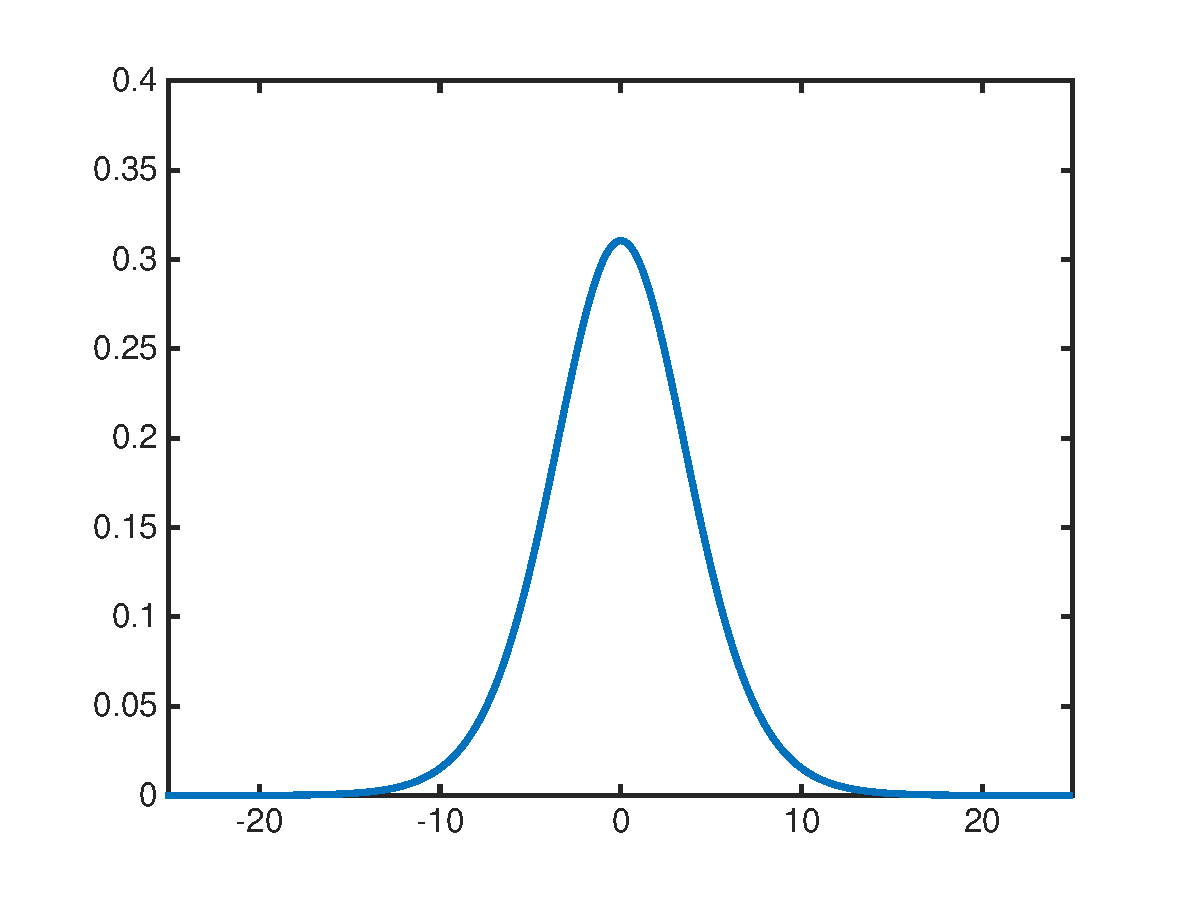
\includegraphics[width=0.48\textwidth]{images/exactsol}
   		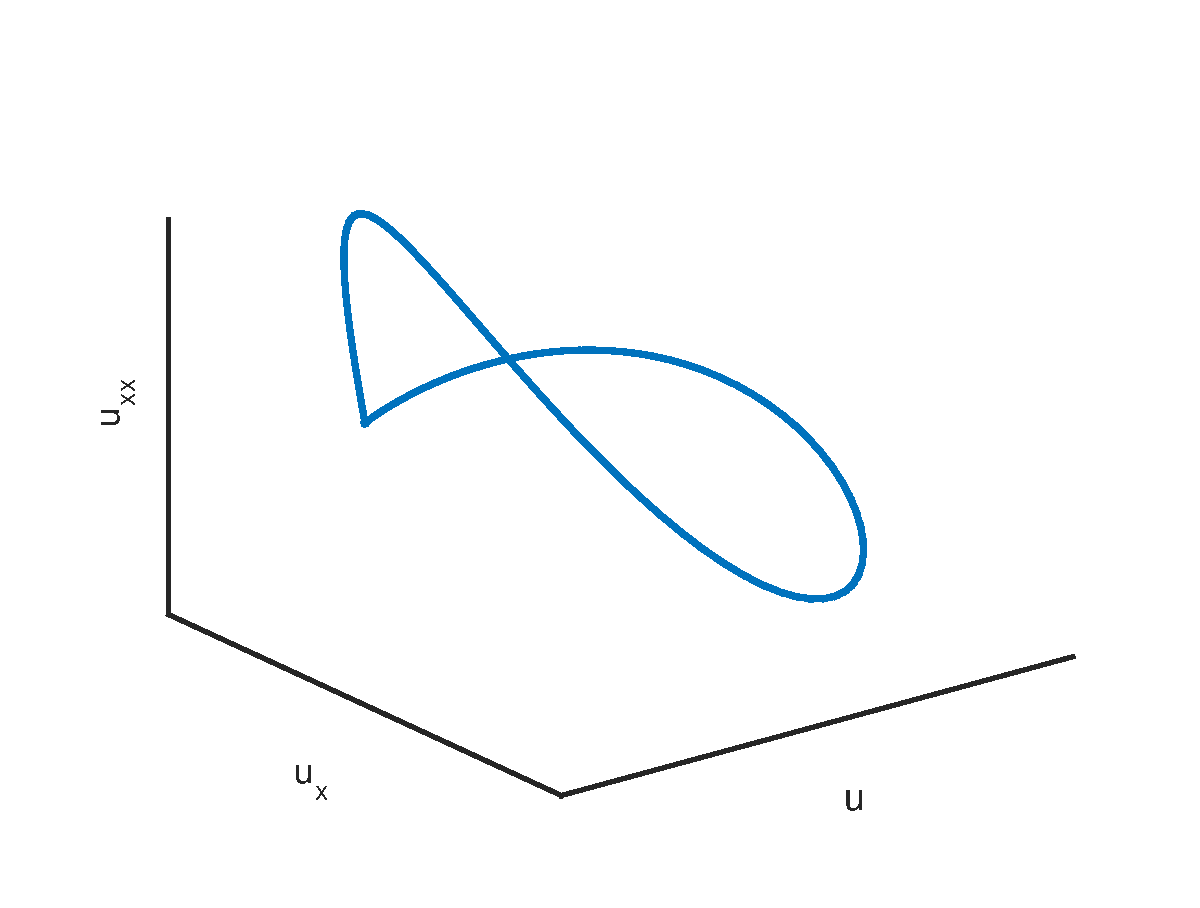
\includegraphics[width=0.48\textwidth]{images/exactsolorbit}
	\end{figure}
\end{frame}

\begin{frame}
\frametitle{Multi-Pulses} 
	\fontsize{14}{7.2}\selectfont
    \begin{block}{Theorem [Buffoni et al. (1996); Sandstede (1997)]}
    For $c > 1/4$, multi-pulse solutions exist, which resemble copies of the primary pulse spliced together.

	\begin{figure}
	\begin{center}
	\includegraphics[width=8cm]{images/multipulse.eps}
	\end{center}
	\end{figure}
	\begin{align*}
	 X_j &\approx \frac{2 \pi}{\beta} k_j + C && k_j \text{ integer}
	\end{align*}

    \end{block}
\end{frame}

\begin{frame}
	\frametitle{Double Pulse Solutions, Numerical Construction}
	\fontsize{16}{7.2}\selectfont
	\begin{figure}
	\begin{center}
	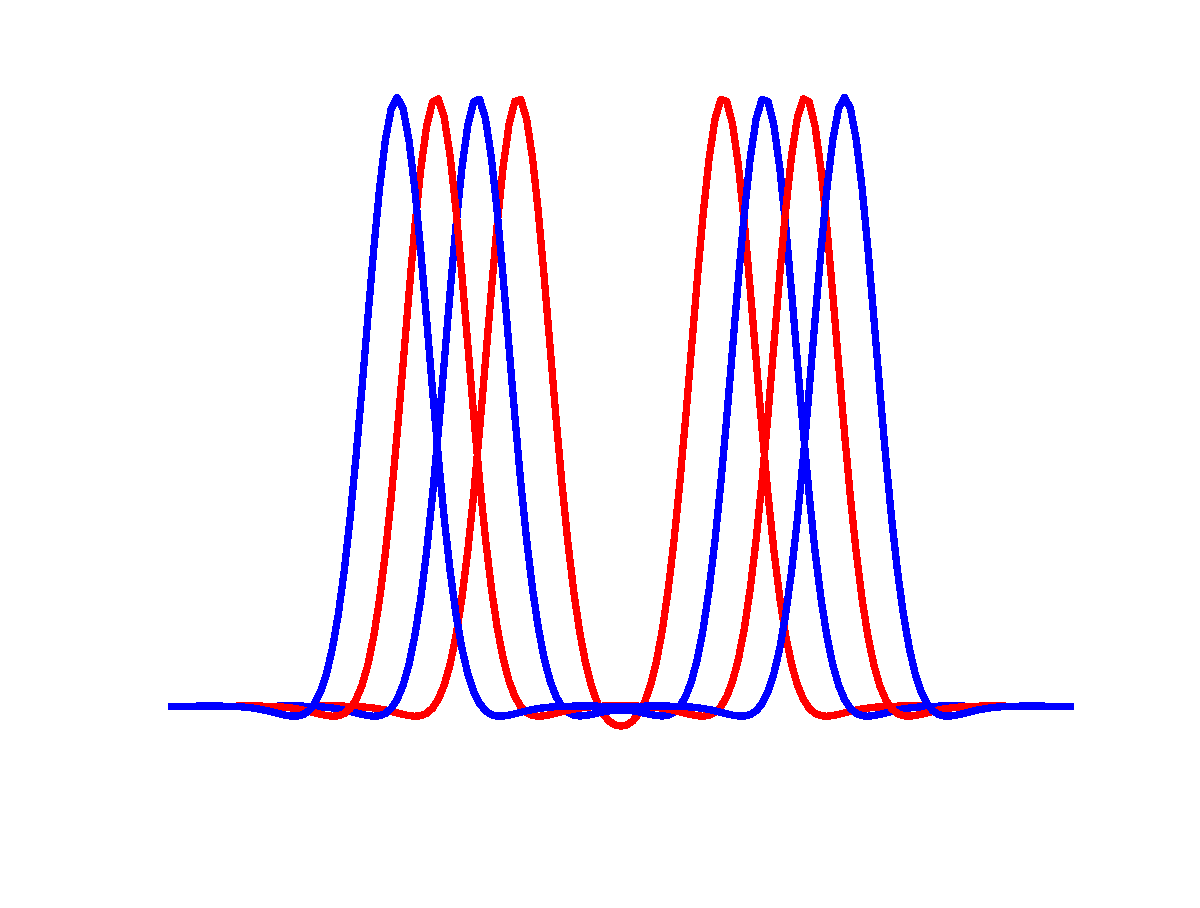
\includegraphics[width=0.7\linewidth]{images/first4dp}
	\end{center}
	\caption{First four double pulses ($c = 10$). \textcolor{red}{$k$ odd}. \textcolor{blue}{$k$ even. } }
	\end{figure}
\end{frame}

\section{Eigenvalue Problem}

\begin{frame}
	\frametitle{Eigenvalue Problem}
	\fontsize{16}{7.2}\selectfont
	Linearization of the PDE about an equilibrium solution $u^*(x)$

	\begin{center}
		$(L - \lambda I )v = 0$
	\end{center}

	\begin{center}
		$L = \partial_x^5 - \partial_x^3 + (c - 2 u^*)\partial_x - 2 u^*_x $
	\end{center}
\end{frame}

\begin{frame}
	\frametitle{Essential Spectrum}
	\fontsize{16}{7.2}\selectfont
	\begin{itemize}
		\item Essential spectrum is entire imaginary axis
			\begin{center}
			\includegraphics[width=0.3\linewidth]{images/essspec1.eps}
			\end{center}

		\item Depends only on background state.
		\vspace{0.5cm}
		\item Independent of solution we are linearizing about.
	\end{itemize}
\end{frame}


\begin{frame}
	\frametitle{Point Spectrum}
	\fontsize{16}{7.2}\selectfont
	\begin{itemize}
		\item Always have double eigenvalue at 0
		\begin{center}
			\includegraphics[width=0.3\linewidth]{images/eigsingle.eps}
		\end{center}
		\item From translation invariance
		\vspace{0.5cm}
		\item Eigenfunctions are $\partial_x u^*$ and $\partial_c u^*$
	\end{itemize}
\end{frame}

\begin{frame}
	\frametitle{Spectrum of Multi-Pulses}
	\fontsize{16}{7.2}\selectfont
	\begin{itemize}
	\item Spectrum of primary pulse
		\begin{center}
			\includegraphics[width=0.2\linewidth]{images/eigsinglepulse.eps}
		\end{center}
	\item For multi-pulses, additional eigenvalues near 0 from interaction between neighboring pulses \footnotesize [Sandstede (1998)]
	\vspace{0.5cm}
	\fontsize{16}{7.2}\selectfont
	\item Interaction eigenvalues must come in quartets
		\begin{center}
			\includegraphics[width=0.8\linewidth]{images/eigdouble2}
		\end{center}
	\end{itemize}
\end{frame}

\begin{frame}
	\frametitle{Spectrum of Double Pulses}
	\begin{center}
		\includegraphics[width=0.8\linewidth]{images/dpsplit}
	\end{center}
\end{frame}

\begin{frame}
	\frametitle{Unstable Double Pulses}
	\begin{center}
		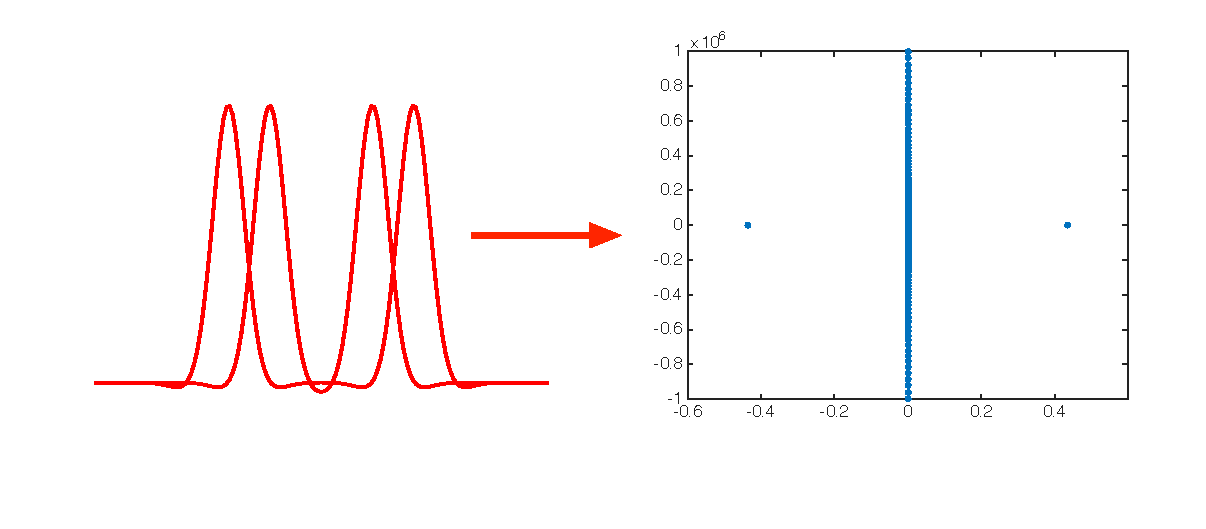
\includegraphics[width=1\linewidth]{images/doubleunstableeig}
	\end{center}
	\begin{itemize}
	\item Pair of real interaction eigenvalues.
	\end{itemize}
\end{frame}

\begin{frame}{Neutrally Stable Double Pulses}
	\begin{center}
		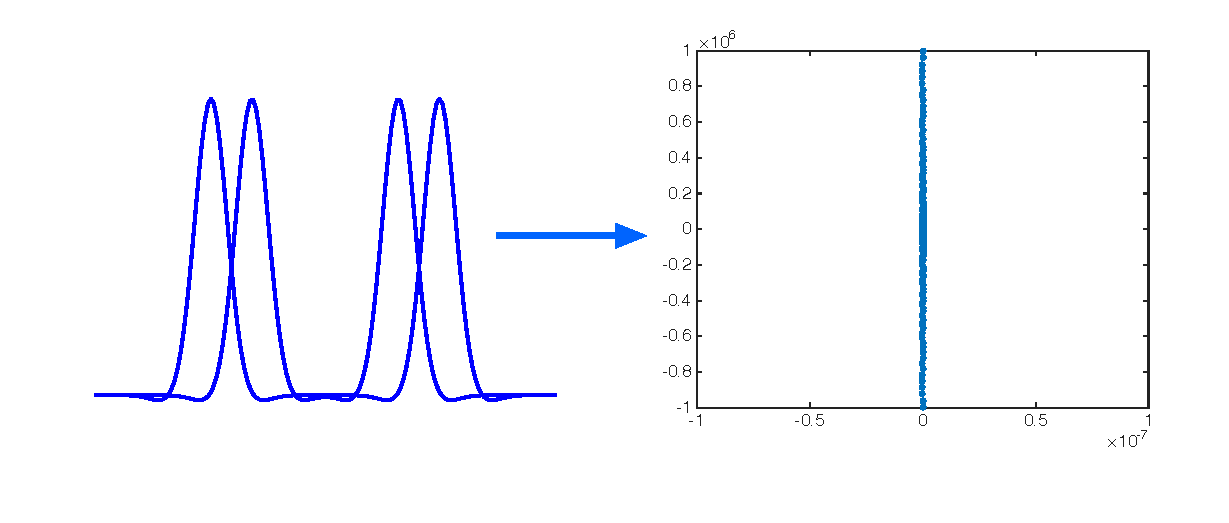
\includegraphics[width=1\linewidth]{images/doublestableeig}
	\end{center}
	\begin{itemize}
	\item Where are the interaction eigenvalues?
	\end{itemize}
\end{frame}

\begin{frame}{Neutrally Stable Double Pulses}
	\begin{center}
		\includegraphics[width=0.5\linewidth]{images/stableeigweighted2}
	\end{center}
	\begin{itemize}
		\item Exponential weight shifts essential spectrum to left
		\item Interaction eigenvalues: $\lambda = \pm \: 2.0829 \times 10^{-11} \pm 0.0691i$
		\item We think interaction eigenvalues are embedded in essential spectrum
		\item Hard to prove since no longer Hamiltonian with exponential weight
	\end{itemize}
\end{frame}

\section{Periodic Multi-Pulses}

\begin{frame}
	\frametitle{Periodic Multi-Pulses}
	\fontsize{16}{7.2}\selectfont
	\begin{itemize}
		\item Essential spectrum becomes discrete
		\vspace{0.5cm}
		\item We don't have to look for embedded eigenvalues
		\vspace{0.5cm}
		\item Each pulse interacts with its two neighbors
		\vspace{0.5cm}
		\item This interaction constrains the allowable pulse distances
		\vspace{0.5cm}
		\item Essential spectrum eigenvalues and interaction eigenvalues can collide
	\end{itemize}
\end{frame}

\begin{frame}
\frametitle{Periodic Multi-Pulses} 
	\fontsize{16}{7.2}\selectfont
    \begin{block}{Theorem}
    For sufficiently well-separated pulses, periodic multi-pulse solutions exist.

	\begin{figure}
	\begin{center}
	\includegraphics[width=8cm]{images/multipulseperiodic2.pdf}
	\end{center}
	\end{figure}
    \end{block}
\end{frame}

\begin{frame}
\frametitle{Periodic Multi-Pulses} 
	\fontsize{16}{7.2}\selectfont
    \begin{block}{Theorem}
    For 2-periodic pulses, solutions with $X_0 \neq X_1$ bifurcate from solutions with $X_0 = X_1$ in a series of pitchforks.

	\begin{figure}
	\begin{center}
	\includegraphics[width=7.25cm]{images/pitchforkdiagram}
	\end{center}
	\end{figure}
    \end{block}
\end{frame}

\begin{frame}
	\frametitle{Location of Eigenvalues}
	\fontsize{16}{7.2}\selectfont
	We expect to find two categories of eigenvalues.

	\begin{itemize}
		\item Discrete ``essential spectrum'' eigenvalues along the imaginary axis.
		\begin{itemize}
			\item Depend only on background state and domain size
			\item Independent of solution we linearize about
		\end{itemize}
		\item Eigenvalues resulting from pulse interaction 
		\begin{itemize}
			\item Each puse interacts with two neighbors
			\item Depend on geometry of periodic multi-pulse
		\end{itemize}
	\end{itemize}
	\vspace{0.5cm}

	By Hamiltonian symmetry, eigenvalues must come in quartets.
\end{frame}

\begin{frame}
\frametitle{Periodic Multi-Pulses} 
	\fontsize{16}{7.2}\selectfont
    \begin{block}{Theorem}
    To leading order, $\lambda$ is a PDE eigenvalue for the linearization about a periodic $n-$pulse if and only if 
    \[
    \det\begin{pmatrix}K(\lambda) & 0 \\ 0 & A - \lambda^2  M I \end{pmatrix} = 0
    \]
    \begin{itemize}
    	\item $K(\lambda)$ is an $n \times n$ matrix which depends only on the background state
    	\item $A$ is an $n \times n$ matrix which depends on the geometry of the $n$-pulse
    \end{itemize}
    \end{block}
\end{frame}

\begin{frame}
	\frametitle{Krein Bubbles}
	\fontsize{16}{7.2}\selectfont
	\begin{itemize}
		\item Potential problem: singular points of the two blocks could overlap.
		\vspace{0.5cm}
		\item What happens when the singular points get close?
		\vspace{0.5cm}
		\item We can try this numerically by going out one of the arms of the pitchfork.

		\begin{figure}
		\begin{center}
		\includegraphics[width=5cm]{images/2pulsepitchfork}
		\end{center}
		\end{figure}
	\end{itemize}
\end{frame}

\begin{frame}
	\frametitle{Krein Bubbles}
	\fontsize{16}{7.2}\selectfont
	\begin{center}
		\includemedia[
		     width=8cm,height=6cm,
		     activate=pageopen,
		     addresource=videos/Kreincollision.mp4,
		     flashvars={
		         source=videos/Kreincollision.mp4
		        &autoPlay=true
		     }
	]{}{VPlayer.swf} 
	\end{center}
\end{frame}

\begin{frame}
	\frametitle{Krein Bubbles}
	\fontsize{16}{7.2}\selectfont
		\begin{figure}
		\begin{center}
		\includegraphics[width=8cm]{images/Kreinbubble1.pdf}
		\end{center}
		\caption{Real part vs. imaginary part of ``essential spectrum'' eigenvalue during Krein bubble.}
		\end{figure}
\end{frame}

\begin{frame}
	\frametitle{Location of Eigenvalues}
	\fontsize{16}{7.2}\selectfont
	\begin{itemize}
		\item Cool stuff.
	\end{itemize}
\end{frame}

\begin{frame}
	\frametitle{Future directions}
	\fontsize{16}{7.2}\selectfont
	\begin{itemize}
		\item Cool stuff.
	\end{itemize}
\end{frame}

\begin{frame}
	\frametitle{References}
	\fontsize{12}{7.2}\selectfont
	\begin{enumerate}
		\item Buffoni B and S\'er\'e E. \emph{A global condition for quasi-random behaviour in a class of conservative systems}. Commun. Pure Appl. Math., 49 (1996), 285-305.
		\item Chugunova M and Pelinovsky P. \emph{Two-pulse solutions in the fifth-order KdV equation: Rigorous theory and numerical approximations}. Discrete and Continuous Dynamical Systems, Series B 8.4 (2007), 773-800.
		\item Groves M D. \emph{Solitary-wave solutions to a class of fifth-order model equations}. Nonlinearity, 11 (1998), 341-353.
		\item Sandstede B. \emph{Verzweigungstheorie homokliner Verdopplungen}. Ph.D. thesis, University of Stuttgart, 1993.
		\item Sandstede B. \emph{Stability of multiple-pulse solutions}. Trans. Am. Math. Soc., 350 (1998), 429-472.
		\item Sandstede B. \emph{Stability of travelling waves}. In: \emph{Handbook of Dynamical Systems II} (B Fiedler, ed). Elsevier (2002) 983-1055.
	\end{enumerate}
\end{frame}
 
\end{document}